\documentclass[a4paper,12pt]{report}

\usepackage{float}
\usepackage[utf8]{inputenc}
\usepackage[margin=1in]{geometry}
\usepackage{url}
\usepackage[backend=bibtex]{biblatex}
\usepackage{commath}
\usepackage{multicol}
\usepackage{graphicx}
\usepackage{pdfpages}

\title{CS699: COVID Combat}
\author{Swarupananda Dhua(22M2102) and Akshat Gautam(190110004)}

\begin{document}

\maketitle

\section{Description of the game}
The name of the Game is “COVID Combat”. It is a 2D game. There is a battlefield consisting of empty places and obstacles through which the active objects (Player and Enemies) of the game can walk and interact. The Player of the Game has an unlimited supply of bullets using which he can kill the enemies. On the other hand, enemies walk randomly and if the Player comes in contact with some enemy, the game is over. If all the enemies are killed, Player wins the game.

\section{What have we achieved TODO}
1.	Grid for the playground has been made.
2.	The Player and Coronaviruses have been added but their behaviours are not yet fully functional.
3.	Sound effects (for background music and player move) have been added.

4. Collision detection between Player and Coronavirus, Shooting Bullets by the Player, Collision Detection between Bullet and Coronavirus.

Following picture is a screenshot of the game:
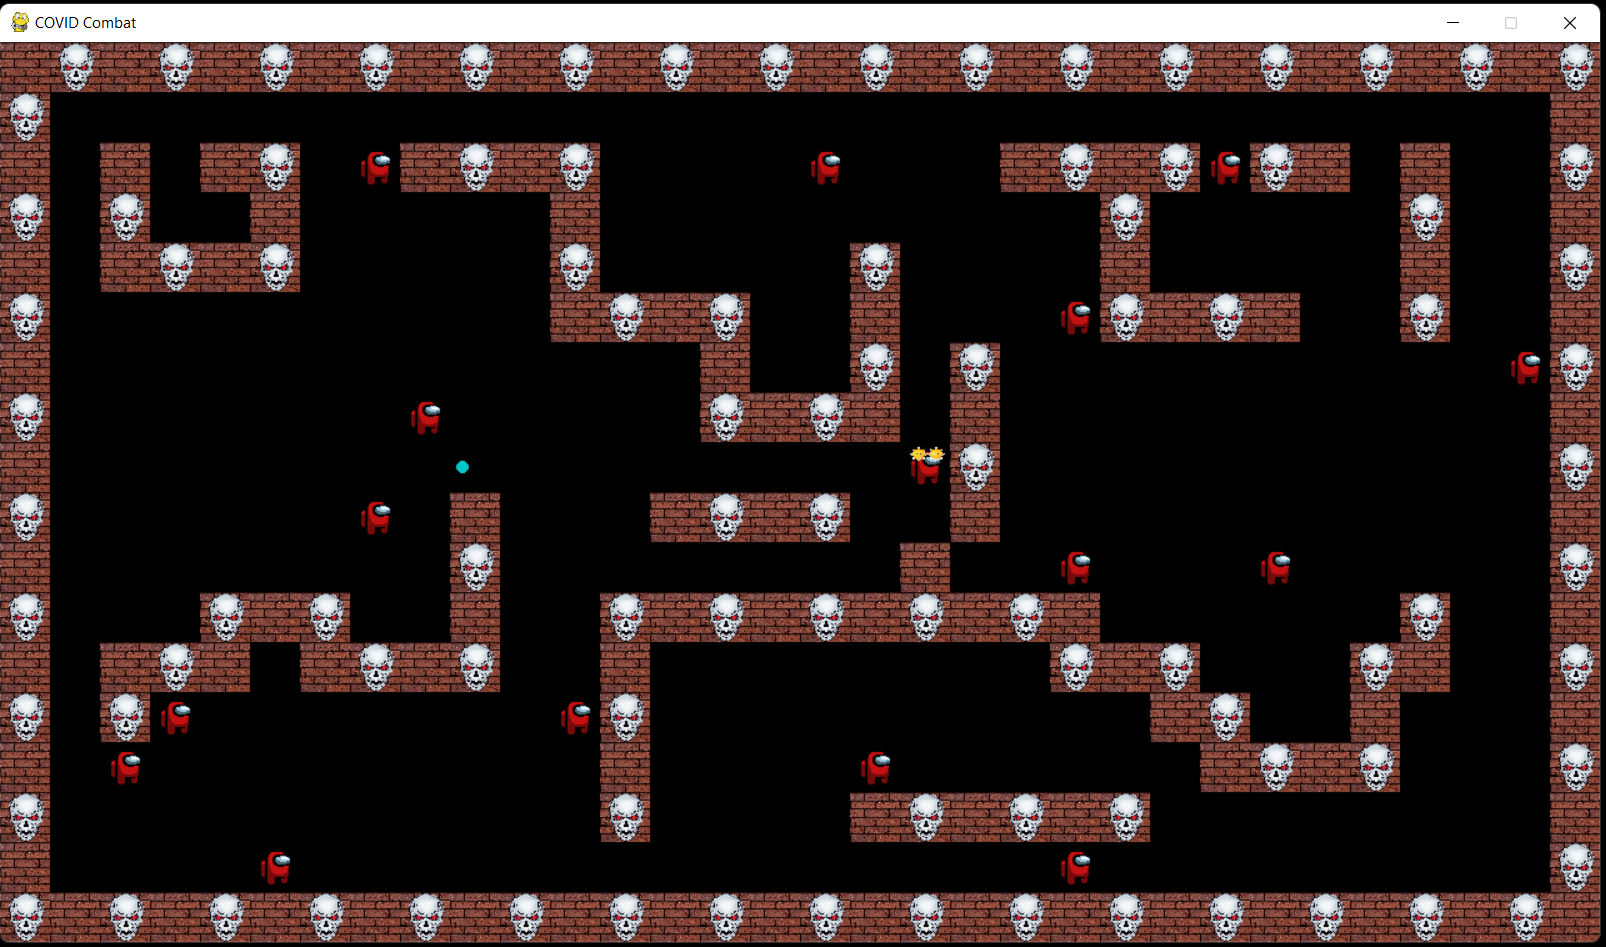
\includegraphics[scale=0.4]{snapshot.png}

\section{Future Work}
In $Camera.py$ we've some experimental code using which we can cast the 2D grid as a 3D scene and convert this game to a pseudo-3D game. We can add other objects such as sky, floor, hills, trees etc. to make the game look better. Also, we can replace the Player and Enemy images by some realistic characters.

\section{Documentation TODO}
Technologies Used: Python and Pygame for coding the logic
Latex for creating user manual/documentation for the game
HTML/CSS for updating the status of the development.

Code structure is as follows:

\section{Running Instructions}
To run this game, you need $python3$ and $pygame$. Installation instructions for $python3$ can be found in $www.python.org$ and for $pygame$ in $www.pygame.org$. Once installed, the game can be run by invoking $python main.py$ from the root directory.

\end{document}